\documentclass[11pt,a4paper]{article}

\usepackage[margin=1in]{geometry}
\usepackage{amsmath}
\usepackage{graphicx}
\usepackage{booktabs}
\usepackage{hyperref}
\usepackage{float}
\usepackage{enumitem}

\graphicspath{{../figures/}}
\hypersetup{
  colorlinks=true,
  linkcolor=blue,
  urlcolor=blue,
  citecolor=blue
}

\title{Signals and Systems Course Project Report}
\author{Generated project draft}
\date{2026 Spring}

\begin{document}
\maketitle

\section{Project Objective}

This project studies basic signal transformations and frequency-domain
analysis using a real audio signal. The sampled audio is denoted by $x[n]$.
Using interpolation, it is treated as an approximation of a continuous-time
signal $x(t)$. The project then analyzes time reversal, time scaling, Fourier
spectra, magnitude-only and phase-only reconstruction, and ideal low-pass
filtering.

\section{Input Audio and MATLAB Environment}

The implementation language is MATLAB. The input audio file is
\texttt{audio/input/original.wav}. It has the following properties:

\begin{itemize}[nosep]
  \item Format: WAV, PCM signed 16-bit little-endian.
  \item Sampling rate: 16000 Hz.
  \item Channels: 1 channel, mono.
  \item Duration: 7.000 seconds.
  \item Preprocessing: amplitude normalization to avoid clipping.
\end{itemize}

The audio is short enough for clear waveform and spectrum plots, but long
enough to show meaningful frequency content.

\section{Interpolation and Continuous-Time Counterpart}

The discrete audio samples $x[n]$ are read by MATLAB using \texttt{audioread}.
To construct a computable approximation of $x(t)$, the project uses linear
interpolation between adjacent samples. In MATLAB this is implemented with
\texttt{interp1}. Figure~\ref{fig:interp} shows the sampled values and the
interpolated curve over a short time window.

\begin{figure}[H]
  \centering
  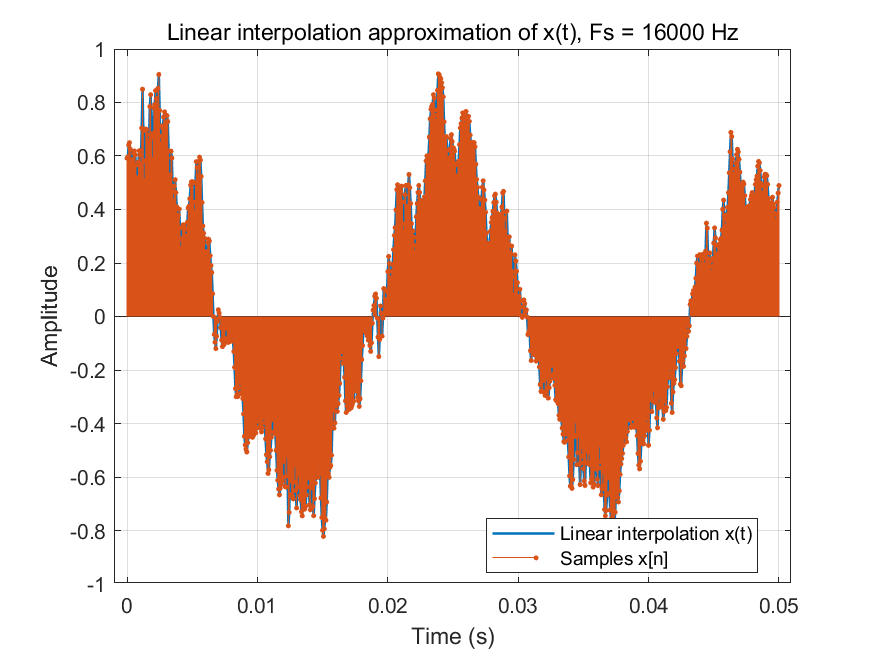
\includegraphics[width=0.85\linewidth]{02_linear_interpolation_xt.png}
  \caption{Linear interpolation approximation of $x(t)$.}
  \label{fig:interp}
\end{figure}

\section{Time-Domain Transformations}

Three time-domain transformations are generated:

\begin{itemize}
  \item $x(-t)$: time reversal, implemented by reversing the audio samples.
  \item $x(2t)$: time compression by a factor of 2. The resulting duration is
  about 3.5 seconds.
  \item $x(t/2)$: time expansion by a factor of 2. The resulting duration is
  about 14 seconds.
\end{itemize}

The time-reversed signal sounds like the original clip played backward. The
compressed signal changes faster in time, while the expanded signal changes
more slowly.

\begin{figure}[H]
  \centering
  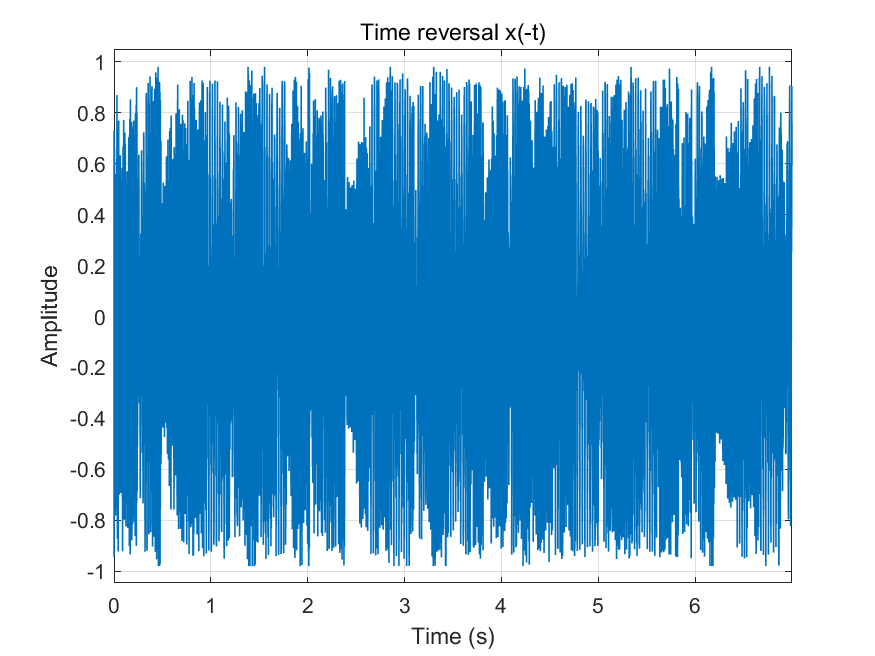
\includegraphics[width=0.95\linewidth]{03_x_reverse_waveform.png}
  \caption{Waveform of $x(-t)$.}
\end{figure}

\begin{figure}[H]
  \centering
  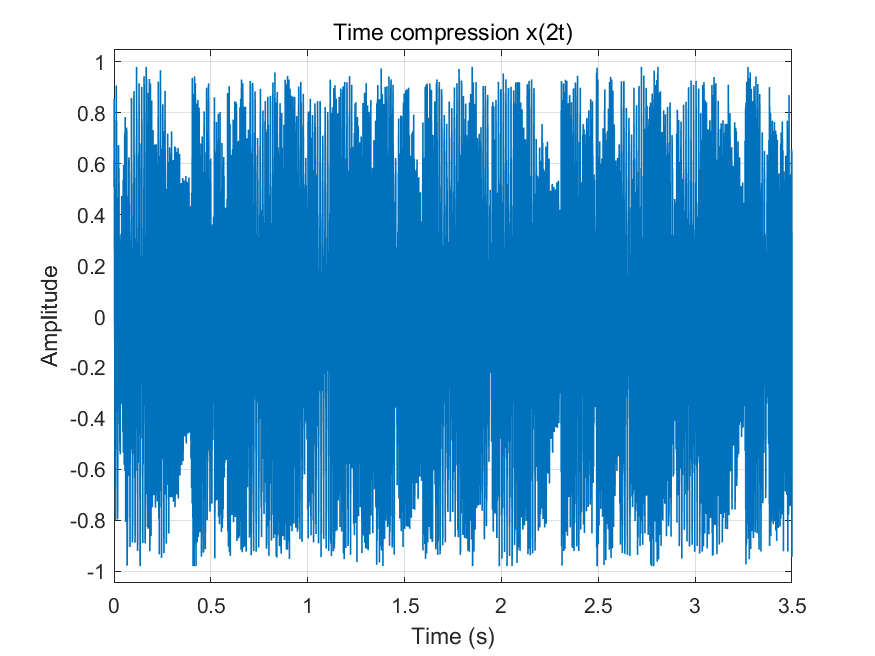
\includegraphics[width=0.95\linewidth]{04_x_2t_waveform.png}
  \caption{Waveform of $x(2t)$.}
\end{figure}

\begin{figure}[H]
  \centering
  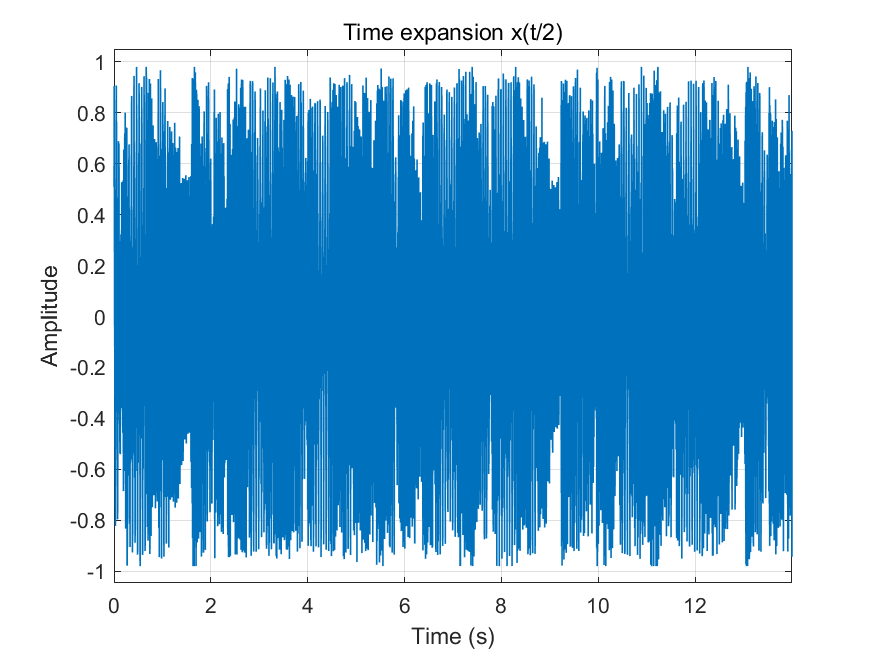
\includegraphics[width=0.95\linewidth]{05_x_t_over_2_waveform.png}
  \caption{Waveform of $x(t/2)$.}
\end{figure}

\section{Fourier Transform and Spectrum Analysis}

The Fourier spectra are computed using the FFT. For visualization,
\texttt{fftshift} places negative frequencies on the left and positive
frequencies on the right. The magnitude spectra are normalized and plotted in
dB.

For time reversal, the magnitude spectrum is largely preserved, while phase is
changed. For $x(2t)$, time compression corresponds to frequency-axis expansion.
For $x(t/2)$, time expansion corresponds to frequency-axis compression. These
observations agree with the Fourier transform time-scaling property:

\[
x(at) \Longleftrightarrow \frac{1}{|a|} X\left(j\frac{\omega}{a}\right).
\]

\begin{figure}[H]
  \centering
  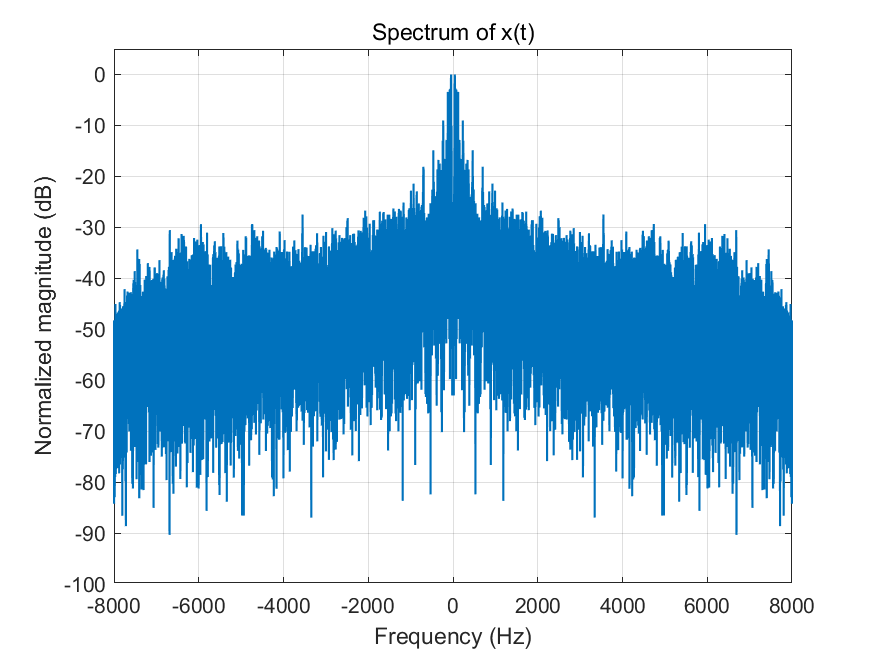
\includegraphics[width=0.95\linewidth]{06_spectrum_original.png}
  \caption{Spectrum of the original signal.}
\end{figure}

\begin{figure}[H]
  \centering
  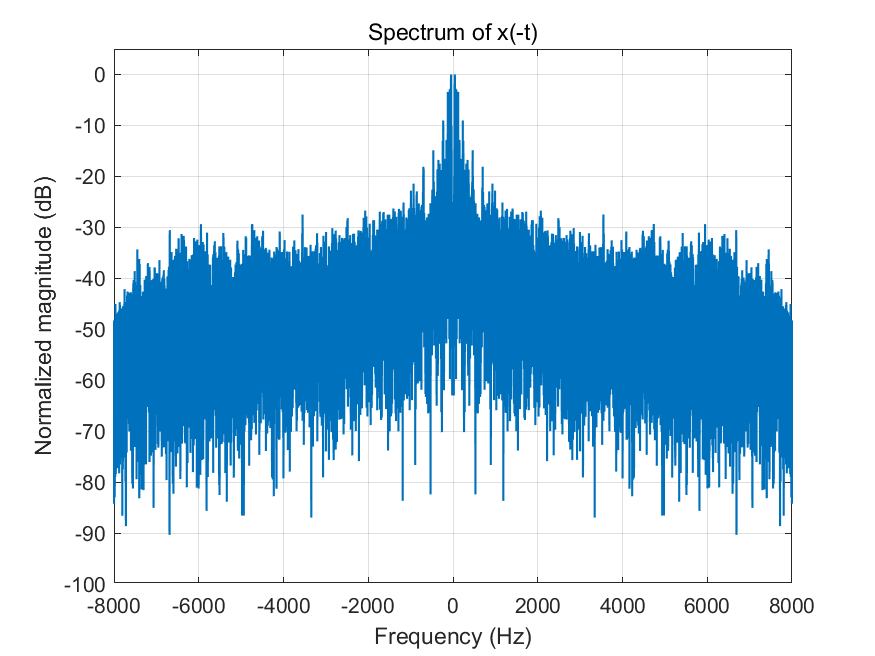
\includegraphics[width=0.95\linewidth]{07_spectrum_x_reverse.png}
  \caption{Spectrum of $x(-t)$.}
\end{figure}

\begin{figure}[H]
  \centering
  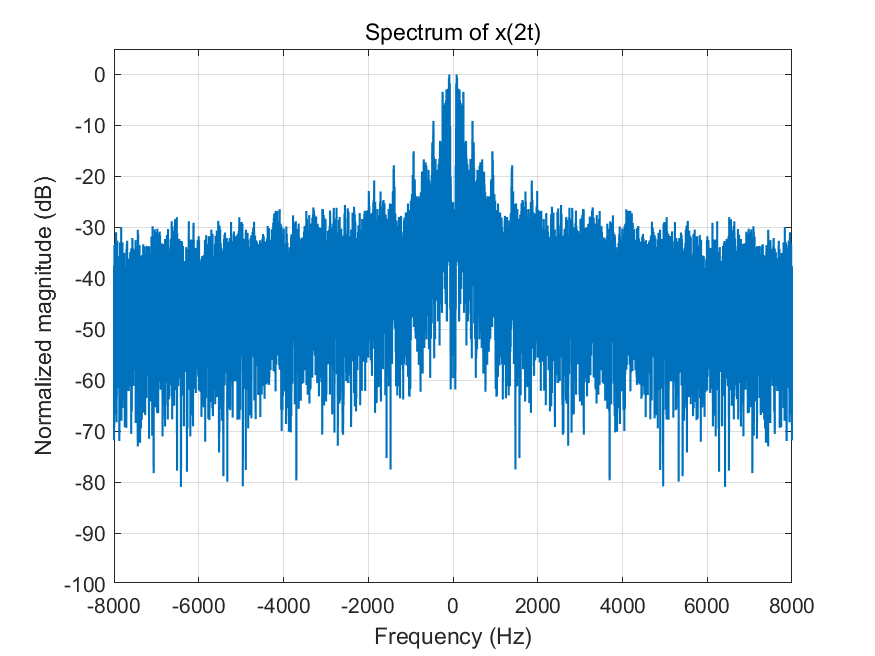
\includegraphics[width=0.95\linewidth]{08_spectrum_x_2t.png}
  \caption{Spectrum of $x(2t)$.}
\end{figure}

\begin{figure}[H]
  \centering
  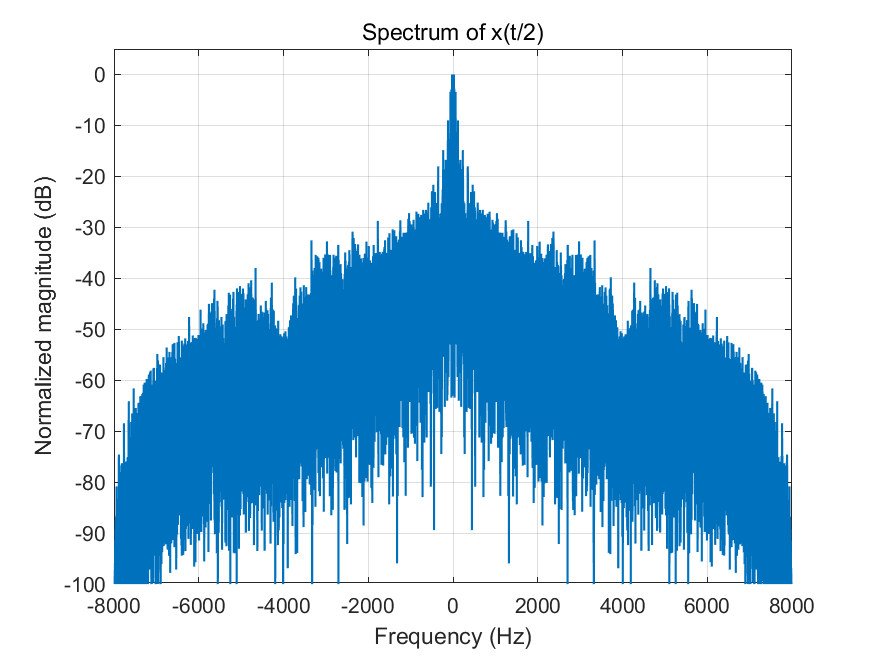
\includegraphics[width=0.95\linewidth]{09_spectrum_x_t_over_2.png}
  \caption{Spectrum of $x(t/2)$.}
\end{figure}

\section{Magnitude-Only and Phase-Only Reconstruction}

Let $X(j\omega)$ be the Fourier transform of $x(t)$. The project compares:

\[
\mathcal{F}^{-1}\{|X(j\omega)|\}
\]

and

\[
\mathcal{F}^{-1}\{e^{j\angle X(j\omega)}\}.
\]

The magnitude-only reconstruction keeps the spectral energy distribution but
throws away phase. The phase-only reconstruction keeps timing and phase
relationships but discards the original magnitude distribution. The resulting
waveforms are very different from the original, showing that both magnitude and
phase are important for reconstructing an audio signal.

\begin{figure}[H]
  \centering
  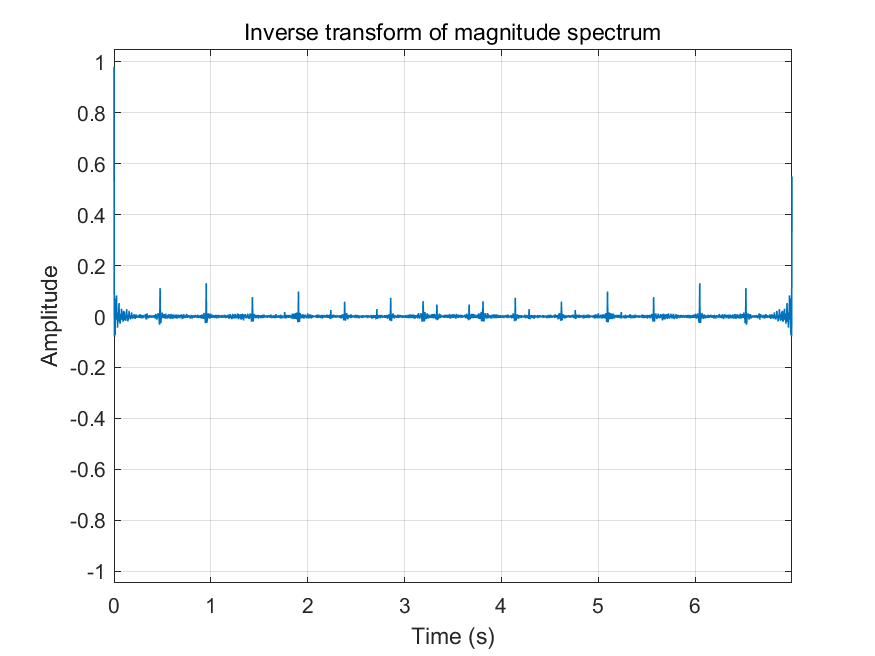
\includegraphics[width=0.95\linewidth]{10_magnitude_only_waveform.png}
  \caption{Inverse transform of the magnitude spectrum.}
\end{figure}

\begin{figure}[H]
  \centering
  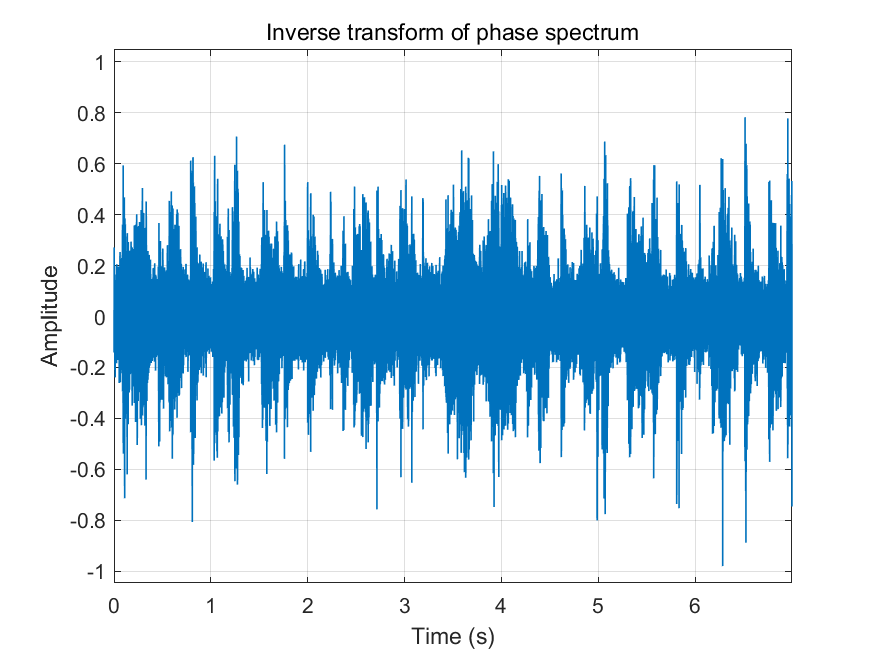
\includegraphics[width=0.95\linewidth]{11_phase_only_waveform.png}
  \caption{Inverse transform of the phase spectrum.}
\end{figure}

\section{Frequency-Domain Low-Pass Filtering}

An ideal low-pass filter is applied in the frequency domain. Since the sampling
rate is 16000 Hz, the Nyquist frequency is 8000 Hz. The chosen cutoff frequency
is 3000 Hz. The filter response is

\[
H(f)=
\begin{cases}
1, & |f|\leq 3000\ \text{Hz},\\
0, & |f|>3000\ \text{Hz}.
\end{cases}
\]

This filter removes high-frequency components while preserving the low and
middle audio band. The filtered waveform and spectrum are shown below.

\begin{figure}[H]
  \centering
  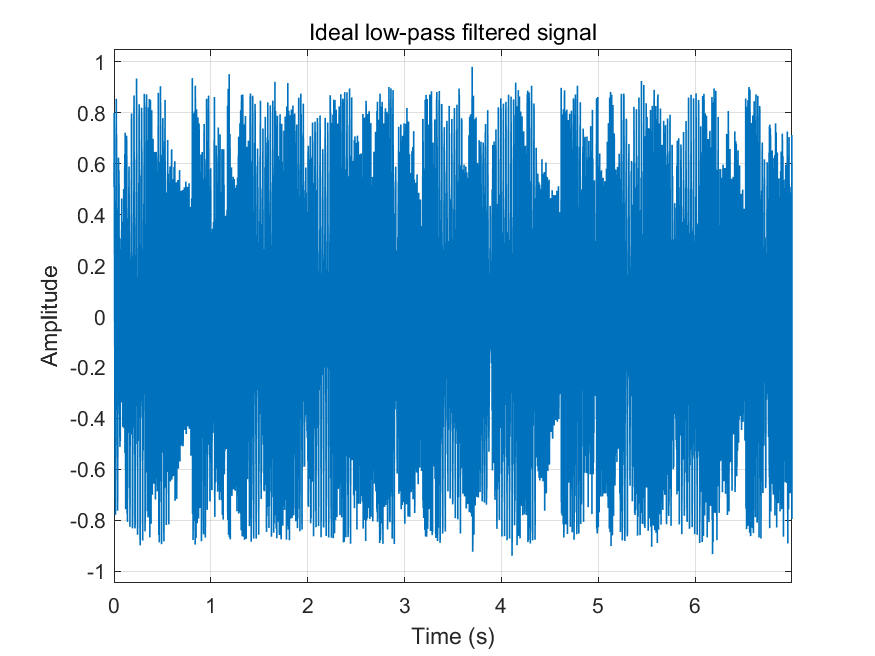
\includegraphics[width=0.95\linewidth]{12_lowpass_waveform.png}
  \caption{Waveform after ideal low-pass filtering.}
\end{figure}

\begin{figure}[H]
  \centering
  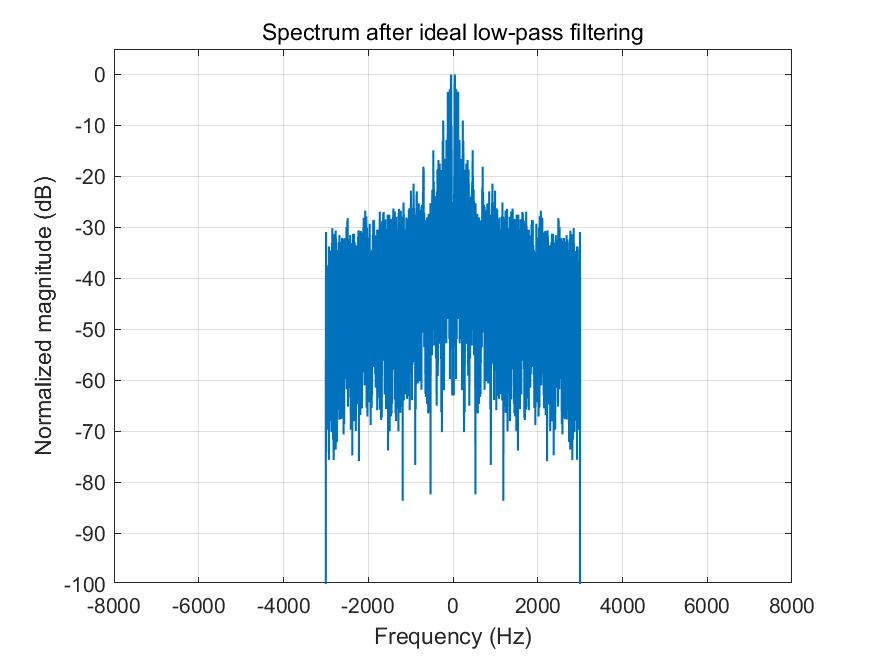
\includegraphics[width=0.95\linewidth]{13_lowpass_spectrum.png}
  \caption{Spectrum after ideal low-pass filtering.}
\end{figure}

\section{Part II: OTFS Paper Study}

The selected paper is \emph{Interference Cancellation and Iterative Detection
for Orthogonal Time Frequency Space Modulation} by P. Raviteja, Khoa T. Phan,
Yi Hong, and Emanuele Viterbo. It was published in IEEE Transactions on
Wireless Communications in 2018. A public preprint is available at
\url{https://arxiv.org/abs/1802.05242}.

The paper studies OTFS modulation over delay-Doppler channels. In high-mobility
scenarios, OFDM can suffer from Doppler spread, which breaks subcarrier
orthogonality and creates inter-carrier interference. OTFS addresses this
problem by placing information symbols in the delay-Doppler domain and then
mapping them to the time-frequency domain for transmission.

The main idea can be translated and summarized as follows. A wireless channel
with multipath delay and Doppler shift has a natural sparse structure in the
delay-Doppler domain. Instead of observing the channel as rapidly changing
subcarriers, OTFS observes it through a two-dimensional representation connected
to physical path delays and velocities. The authors derive an input-output
relationship for OTFS modulation and demodulation, analyze the resulting
interference, and propose a message-passing detector that iteratively cancels
interference and estimates the transmitted symbols.

OTFS can overcome frequency-selective fading because multipath delays are
represented explicitly along the delay dimension. It can also handle fast
mobility because Doppler shifts are represented explicitly along the Doppler
dimension. Since practical wireless channels often contain only a limited number
of dominant propagation paths, the delay-Doppler representation is sparse. This
sparsity makes joint detection and interference cancellation practical.
Therefore, OTFS is more robust than conventional OFDM in channels with severe
time variation and Doppler spread.

\section{Generated Files}

\begin{table}[H]
\centering
\begin{tabular}{ll}
\toprule
File & Meaning \\
\midrule
\texttt{audio/output/original\_normalized.wav} & Normalized source audio \\
\texttt{audio/output/x\_reverse.wav} & Time reversal $x(-t)$ \\
\texttt{audio/output/x\_2t.wav} & Time compression $x(2t)$ \\
\texttt{audio/output/x\_t\_over\_2.wav} & Time expansion $x(t/2)$ \\
\texttt{audio/output/magnitude\_only\_reconstruction.wav} & Magnitude-only reconstruction \\
\texttt{audio/output/phase\_only\_reconstruction.wav} & Phase-only reconstruction \\
\texttt{audio/output/lowpass\_ideal\_3000Hz.wav} & Ideal low-pass result \\
\bottomrule
\end{tabular}
\caption{Generated audio files.}
\end{table}

\section{Conclusion}

The MATLAB implementation completes all signal-processing requirements of the
project. The experiments demonstrate how time-domain transformations affect
both waveform duration and spectral distribution, why magnitude and phase are
both necessary for faithful reconstruction, and how frequency-domain filtering
can be implemented through the Fourier transform. The OTFS paper study further
connects transform-domain signal characterization with modern wireless
communication systems.

\end{document}
